\section{Stationary Extremes}\label{sec:statio}

From now, we considered the maximum $X_{(n)}=\max_{1\leq i\leq n}X_i$ composed of independent random variables only. 
 Now, we are interested by modeling 
$X^*_{(n)}=\max_{1\leq i\leq n}X^*_i$ where $\{X^*_i\}$ will now denote a \emph{stationary} 
sequence of $n$ random variables sharing the same marginal df as the sequence $\{X_i\}$ of independent random variables, $F$.

\begin{definition}[Stationary process] We say that the sequence $\{X_i\}$ of n random variables is (strongly) \emph{\textbf{stationary}} if, for $h\geq 0$ and $n\geq 1$, the distribution of the lagged random vector $(X_{1+h},\dots,X_{n+h})$ does not depend on h.
\end{definition}
It corresponds to physical processes whose stochastic properties are homogeneous but which may be dependent. This dependence can take many forms and hence we need to relax the independence condition.
Let's denote $F_{i_1,\dots,i_p}(u_1,\dots,u_p):=\text{Pr}\{X_{i_1}\leq 
u_1,\dots,X_{i_p}\leq u_p\}$ the joint df of 
$X_{i_1},\dots,X_{i_p}$ for any arbitrary positive integers $(i_1,\dots,i_p)$.

\begin{definition}[$D(u_n)$ dependence condition from \cite{leadbetter_extreme_1974}] 
	Let $\{u_n\}$ be a sequence of real numbers. We say that the \emph{ \boldsymbol {$D(u_n)$} \textbf{condition}} holds if for any set of integers $i_1<\dots<i_p$ and $j_1<\dots<j_q$ such that $j_1-i_p>\ell$, we have that 
	
	\begin{equation}
	|F_{i_1,\dots,i_p,j_1,\dots,j_q}(u_n,\dots,u_n;u_n,\dots u_n)-F_{i_1,\dots,i_p}(u_n,\dots,u_n)\cdot F_{j_1,\dots,j_q}(u_n,\dots u_n)|\leq \beta_{n,\ell}\ ,
	\end{equation}
	where $\beta_{n,\ell}$ is nondecreasing and  $\displaystyle{\lim_{n \to \infty}}\beta_{n,\ell_n}=0$ for some sequence $\ell_n=o(n)$.
\end{definition}
This condition ensures that, when the sets of variables are separated by a relatively short distance, typically $s_n=o(n)$, the long-range dependence between such events is limited in a sense that is sufficiently close to zero to have no effect on the limit extremal laws.
This result is remarkable in the sense that, provided a series has limited long-range dependence at extreme levels (i.e., where $D(u_n)$ condition holds), maxima of stationary series follow the same distributional limit laws as those of independent series. The two following theorems will show the main implications.


\begin{theorem}[Limit distribution of maxima under $D({u_n})$, \cite{leadbetter_extreme_1974}]
	Let $\{X^*_i\}$ be a stationary sequence of $n$ iid random variables. If there exists sequences of constants $\{a_n>0\}$ and $\{b_n\}$ such that $D(u_n)$ condition is satisfied with $u_n=a_nx+b_n$ for every real $x$, and	
	\begin{equation}
	\text{Pr}\{X^*_{(n)}\leq u_n\}\longrightarrow G^*(x), \ \ \ \ \ \ \ \, \ \ n\rightarrow\infty,
	\end{equation}
	where $G$ is a non-degenerate df, then $G^*$ is a member of the GEV family as presented in \hyperref[extthm]{Theorem \textbf{\ref{extthm}}}.
	
\end{theorem}


\begin{theorem}[\citet{leadbetter_extremes_1983}]\label{thm:statio2}
	Let $\{X^*_i\}$ be a stationary sequence and let $\{X_i\}$ be a sequence of iid random variables. We have under regularity conditions, 
	\begin{equation*}
	\text{\emph{Pr}}\big\{a_n^{-1}(X_{(n)}-b_n)\leq x\big\}\longrightarrow G(x), \ \ \ \ \ \ \ \ \ \ \ n\rightarrow \infty,
	\end{equation*}
	for normalizing sequences $\{a_n>0\}$ and $\{b_n\}$, where $G$ is non-degenrate, if and only if 
	
	\begin{equation*}\label{extremindex}
	\text{\emph{Pr}}\big\{a_n^{-1}(X^*_{(n)}-b_n)\leq x \big\}\longrightarrow G^*(x), \ \ \ \ \ \ \ \ \ \ \  n\rightarrow\infty,
	\end{equation*}
	where $G^*$ is the limit df coming from a stationary process, defined by
	
	\begin{equation}\label{extindex}
	G^*(x)=G^{\theta}(x),
	\end{equation}
	for some constant $\theta\in (0,1]$ called the \emph{\textbf{extremal index}}.
	
\end{theorem}
It is evident from (\ref{extindex}) that the maximum of a stationary series will have a tendency to decrease.

\subsection{The extremal index}
The \emph{extremal index} is an important indicator quantifying the extent of extremal dependence, that is the degree at which the assumption of independence is violated. From (\ref{extindex}), it is clear that $\theta=1$ lead to an independent process, but the converse does not hold. The case $\theta= 0$ will not be considered as it is too "far" from independence and brings problems. Moreover, the results of \hyperref[thm:statio2]{Theorem \textbf{\ref{thm:statio2}}} would not hold.

Formally, it can be defined as

\begin{equation}\label{exc}
\theta=\displaystyle{\lim_{n \to \infty}}\text{Pr}\big\{\max(X_2,\dots,X_{p_n})\leq u_n\ | \ X_1\geq u_n\big\},
\end{equation}
in the POT approach, where $p_n=o(n)$ and the sequence $u_n$ is such that Pr$\big\{X_{(n)} \leq u_n\big\}$ converges.
Hence, $\theta$ can be thought for example as the probability that an exceedance over a high threshold is the final element in a \textit{cluster} of exceedances (defined in the following subsection).



\addcontentsline{toc}{subsubsection}{New parameters}
\subsubsection*{New parameters}
 When $0<\theta\leq 1$, we have from \hyperref[thm:statio2]{Theorem \textbf{\ref{thm:statio2}}} that $G^*$ is an EV distribution but with different scale and location parameters than $G$. If we note by ($\mu^*,\sigma^*,\xi^*$) the parameters pertaining to $G^*$ and those from $G$ kept in the usual way, we have the following relationships, when $\xi\neq 0$

\begin{equation}
\mu^* = \mu-\sigma\xi^{-1}(1-\theta^{\xi}), \ \ \ \   \ \text{and} \ \quad \sigma^*=\sigma\theta^{\xi}.
\end{equation}
In the Gumbel case ($\xi=0$), we simply have $\sigma^*=\sigma$ and $\mu^*=\mu+\log\theta$.
The fact that $\xi^*=\xi$ induce that the two distributions $G^*$ and $G$ will have the same form, following \hyperref[thm:statio2]{Theorem \textbf{\ref{thm:statio2}}}.



\addcontentsline{toc}{subsubsection}{Clusters of exceedances}
\subsubsection*{Clusters of exceedances}

 From (\ref{exc}) and in a POT context, extremes have the tendency to occur in cluster whose \emph{mean cluster size} is $\theta^{-1}$ at the limit. Equivalently, $\theta^{-1}$ can be viewed as the factor with which the mean distance between cluster is increased.
This problem of temporal dependence make inference based on the likelihood invalid.
We name two methods that can be used to circumvent this issue : 

\begin{itemize}
	\item \textbf{Filtering out} an (approximate) independent sequence of threshold exceedances.
	\item \textbf{Declustering} : compute the maximum value in each cluster and then we model these clusters maximums as independent GP random variable. In this approach, we remove temporal dependence but we do not estimate it.
	However, information is discarded and this could be a substantial loss in meteorological applications, for instance to determine heat or cold waves.
\end{itemize}



\addcontentsline{toc}{subsubsection}{Return levels}
\subsubsection*{Return levels}

Because of clustering, notion of return level is more complex and the dependence appear in the definition of return levels for excess models :

\begin{equation}\label{eq:rlstatio}
r_m = u + \sigma\xi^{-1}\Big[(m\zeta_u\theta)^{\xi}-1\Big].
\end{equation}
Hence, we see that ignoring dependence will lead to an overestimation of return levels. For example, we have that :

\begin{itemize}
	\item If $\theta=1$, then the \textit{100-year-event} has probability 0.368 of not appearing in the next 100 years.
	\item If $\theta=0.1$, the event has probability of 0.904 of not appearing in the next 100 years.
\end{itemize}


\subsection{Modelling in Block Maxima}

With dependent series, modeling by means of GEV as in 
\hyperref[sec::1]{Chapter \textbf{\ref{sec::1}}} can be used in 
a similar way from the fact that the shape parameter $\xi^*$ will remain invariant. The difference is that the effective number of block maxima $n^*=n\theta$ will be reduced and hence convergence in \hyperref[extthm]{extremal Theorem \textbf{\ref{extthm}}} will be slower. 
Indeed, effective number of observations will be reduced from $n$ to $n\theta$, approximation is expected to be poorer and this will be exacerbated with increased levels of dependence in the series.
Efforts must be made to either try to increase $n$ for example by reducing the blog length, or make sure the model fit is convincing with tools presented in \hyperref[sec:diag]{Section \textbf{\ref{sec:diag}}}.


\section{Non-Stationary Extremes}\label{nstatio}

Whereas \hyperref[sec:statio]{previous Section} relaxed the first "i" of the "iid" assumption made during the whole \hyperref[sec::1]{Chapter \textbf{\ref{sec::1}}} by allowing temporal dependence under stationary process, this section will now tackle the "\textbf{id}", i.e. assumption that the observations are \textbf{i}dentically \textbf{d}istributed. 
Following \cite{milly_climate_2008}, the stationarity assumption is not likely to hold for climatological data such as temperatures. For instance, the most obvious departure from stationarity is the presence seasonal patterns as seen in Figure \ref{fig:violin_density} as there is higher variance in spring or autumn for example. However, seasonal concerns should disappear for very high thresholds in excess models and for a sufficiently large block size in block maxima. Furthermore, the aim of this thesis is to assess 


\begin{itemize}
	\item Positive trend
	\item Seasonality
\end{itemize}

The aim of our modeling will more focus on a different parametrization for the mean, thus in allowing the location parameter $\mu$ to vary through time.

No such general theory as in previous section can be established for non-stationary processes and we will then use a pragmatic approach of combining standard EV models with statistical modeling.

\subsection{Block-Maxima}

As we continue to consider modeling data in yearly blocks, we do only face nonstationary concerns for the trend which is (probably) imputed to the Global Warming. 
The evidence of seasonality arising when we decrease the length of the blocks is not an issue for yearly modeling. However, we loose information, or comparatively, we do not use all the information as at least one half 


\subsubsection*{Inference for GEV}

In order to do inference in a nonstationary context, maximum likelihood is preferred for its adaptability to changes in model structure. In a general setting, we let a nonstationary GEV model to describe the distribution $Z_t$ for $t=1,\ldots,m$ :

\begin{equation}\label{eq:gevnsta}
Z_t\sim \text{GEV}\big(\mu(t), \sigma(t),\xi(t)\big),
\end{equation}
where each of $\mu(t),\sigma(t), \xi(t)$ have an expression of the form
\begin{equation}\label{eq:linknsta}
\theta(t)=b\big(X^{'}\beta\big)
\end{equation}
for a specified (inverse link) function $b(\cdot)$ where $\theta$ denotes either $\mu,\sigma$ or $\xi$ and where $\beta$ denote the complete vector of parameters. In our example, $Z_t$ will describe the annual maximum temperatures for $m=116$ years.
As stated above (?) it will not be recommended to allow $\xi$ to vary with time. Examples of parametric expressions from (\ref{eq:linknsta}) will be given in \hyperref[sec:comp0]{Section \textbf{\ref{sec:comp0}}}.

If $g\big(z_t; \mu(t),\sigma(t),\xi(t)\big)$ denotes the GEV density (Table \ref{tab:gevdens}) with parameters $\mu(t),\sigma(t),\xi(t)$ evaluated at $z_t$, the log-likelihood of the model (\ref{eq:gevnsta}) is, provided $\xi(t)\neq0 \ \forall t$,
\begin{equation}\label{eq:loglikgevnonstatio}
\begin{aligned}
\ell(\beta)& = \sum_t^m\log g\big(z_t; \mu(t),\sigma(t),\xi(t)\big)\\ & = -\sum_t^m\Bigg\{ \log\sigma(t)+\big[1+\xi^{-1}(t)\big]\log\bigg[1+\xi(t)\cdot\sigma^{-1}(t)\cdot\Big(z_t-\mu(t)\Big)\bigg]_+ \\ & \qquad\qquad\qquad\qquad\qquad\qquad\qquad\quad +  \bigg[1+\xi(t)\cdot\sigma^{-1}(t)\cdot\Big(z_t-\mu(t)\Big)\bigg]_+^{-\xi^{-1}(t)} \Bigg\},
\end{aligned}
\end{equation}
where the notation  $y_+(t)=\text{max}\big\{y(t),0\big\}$ holds for $t=1,\ldots,m$. The parameters $\mu(t),\sigma(t),\xi(t)$ are replaced by their respective expressions from (\ref{eq:linknsta}). Note that if $\xi(t)=0$ for any $t$, we must replace the likelihood by using the limit $\xi(t)\to0$ in (\ref{eq:loglikgevnonstatio}) as in Table \ref{gevdens}. 
Numerical techniques are then used to maximize (\ref{eq:loglikgevnonstatio}) to yield the MLE of $\beta$ and evaluate standard errors.  



\subsection{Model Comparisons}

In order to compare our models, that is for example to check whether a trend is statistically significant, or if the nonstationnary models provide an improvement over the simpler (stationary) model, we will use two techniques :

\begin{enumerate}
	\item The \emph{deviance statistic} which is defined as 
	\begin{equation}
	D = 2\big\{\ell_1(\mathcal{M}_1)-\ell_0(\mathcal{M}_0)\big\},
	\end{equation}
	for two nested models $\mathcal{M}_0\subset \mathcal{M}_1$, where $\ell_1(\mathcal{M}_1)$ and $\ell_0(\mathcal{M}_0)$ are the maximized log-likelihoods under models $\mathcal{M}_1$ and $\mathcal{M}_0$ respectively as defined in .
	Asymptotically, the distribution of $D$ is $\chi^2_k$ with $k$ degrees of freedom (df) representing the difference of parameters between model $\mathcal{M}_1$ and $\mathcal{M}_0$. Comparisons of $D$ with the critical values from $\chi_k$ will guide our decision.
	We will use this technique in the \hyperref[sec:comp0]{next Section} to make successive comparisons of parametric models that we propose for the trend.  
	
	\item It is sometimes preferable to rely on other criterion, for example when the number of models to be compared is large or their construction is not straightforward. We will make use of the \emph{Bayesian Information Criterion} (BIC) and  the \emph{Akaike Information Criterion (corrected) } ($\text{AIC}_{\text{c}}$). Used by \citet{cannon_flexible_2010}, these two criterion both have a likelihood term which represent the quality of fit of the model and a term which penalizes the complexity of the model represented by its number of parameters to be estimated. These two criterion are advised for small samples and to prevent overfitting (i.e., fitting to noise instead of the true underlying process), but BIC will penalize more heavily models that are more complex.
	
\end{enumerate}
The basic principle of parsimony holds for both methods. In the first method, it is incorporated in the statistical test since the critical value $\chi^2_k$ will increase with $k$ the difference of complexity of two models and in the second method it is directly included in the criterion.

We will then summarize all the results in the Table \ref{tab:comp_mod} in the \hyperref[sec:nnxp]{following Section} by means of the BIC and $\text{AIC}_{\text{c}}$, \textbf{taking all the models into account.}



\subsubsection*{Model Diagnostics}

After




\section{Return Levels : New Definitions}\label{sec:returnlvlnstatio}

Whereas we already defined return levels in \hyperref[rlgev]{Section  \textbf{\ref{rlgev}}} for independent sequences, we will now give a more general definition for return periods. 

\subsubsection*{Stationarity} 
Under assumption of a
stationary sequence, the return level is the same for all years. The $m$-year return level $r_m$ is associated with a return period of $m$ years. Let $X_{(n),y}$ denote the annual maximum for a particular year $y$. Assuming $\{X_{(n),y}\}\stackrel{iid}{\sim}F$, there are two main interpretations for return periods in this context, following \citet[chap.4]{ag_extremes_2013} :

\begin{enumerate}
	\item \textbf{Expected waiting time until an exceedance occurs :} let $T$ be the year of the first exceedance. Recalling $F(r_m) = \text{Pr} \big\{X_{(n),y}\leq r_m\big\}=1-1/m$, we write
	
	\begin{equation*}
	\begin{aligned}
	\text{Pr}\{T=t\}=\  & \text{Pr}\{X_{(n),1}\leq r_m,\dots,X_{(n),t-1}\leq r_m,X_{(n),t}>r_m\} \\
	=\ & \text{Pr}\{X_{(n),1}\leq r_m\}\dots\text{Pr}\{X_{(n),t-1}\leq r_m\}\text{Pr}\{X_{(n),t}>r_m\}&  \quad  \boxed{\textnormal{iid assumption}}\\
	= \ & \text{Pr}\{X_{(n),1}\leq r_m\}^{t-1}\ \text{Pr}\{X_{(n),1}>r_m\} &  \quad \boxed{\text{ stationarity}}\\
	=\ & F^{t-1}(r_m)(1-F(r_m))\\
	=\ & (1-1/m)^{t-1}(1/m).
	\end{aligned}
	\end{equation*}
	We easily recognize that $T$ has a geometric distribution with parameter $1/m$. Hence, its expected value is $1/m^{-1}$, showing that the expected waiting time for an $m$-year event is $m$ years.
	
	\item \textbf{Expected number of events in a period of \boldsymbol{$m$} years is exactly 1 :} to see that, we define  
	
	\begin{equation*}N=\sum_{y=1}^m \mathbb{I}(X_{(n),y}>r_m)
	\end{equation*}
	as the random variable representing the number of exceedances in $m$ years, with $\mathbb{I}$ the indicator function. Hence, each year is a "trial", and from the fact that \big\{$X_{(n),y}$\big\} are iid, we can compute the probability that the number of exceedances in $m$-years is $k$
	\begin{equation*}
	\text{Pr}\{N=k\}=\binom{m}{k}(1/m)^k(1-1/m)^{m-k},
	\end{equation*}
	where we retrieve $N\sim \ \text{Bin}(m,1/m)$ and hence $N$ has an expected value of $m\cdot m^{-1}=1$.
	
\end{enumerate}


\subsubsection*{Non-stationarity}

As demonstrated in \citet[Section 4.2]{ag_extremes_2013}, we can retrieve the same two interpretations of return period as for a stationary process. However, mathematical derivations go beyond the scope of this thesis. Moreover, from definition of non-stationary process, as parameter(s) will be function of time, return levels will also change over time. This will have big impacts on modeling, since an inappropriate model will lead to inappropriate return levels, see for example Figure ??? . 
Hence, we will now try more complex models in order to improve this fit. 


\section{Neural Networks to Model Nonstationary Series}

In the era of Artificial Intelligence (AI) and Machine Learning, or more precisely of Artificial Neural Networks (ANN) or the trendy term \textit{Deep Learning}, it is interesting to study how this complex mechanism works and how it can be efficiently applied to deal with the issue of nonstationarity in EVT that we confront.


In practice, the assumption of linearity (or the basic functions we  tested) we have hold may not be appropriate enough, in the sense that it could not take the complex temporal relationship of the whole maximum temperature process. \citet{kharin_estimating_2005-1} allowed for nonlinear trends in temperature extremes in another fashion : they made simulations over a 110-year transient global climate to estimate linear trends in the three GEV parameters based on a series of overlapping 51-year time windows.

While this modelling allows for much more flexibility, we keep in mind that it will also be detrimental for the understanding of the "structure" of this relationship

\subsection{Generalized Likelihood Methods}
introduced by \citet{martin_generalized_2000}
In \hyperref[likgevintro]{Section \textbf{\ref{likgevintro}}} we introduced the concept of penalized likelihood (see \citet{coles_likelihood-based_1999}). The idea is that The MLE's may diverge, especially when sample size is small. To resolve this problem, suggest the use of a prior distribution for the shape parameter of the GEV model such
that the most probable values of the parameter are included.

When dealing with nonstationnary processes, it is interesting to consider Generalized Maximum Likelihood (GML) estimators. In this case, \cite{Adlouni_generalized_2007} have proven that GML is likely to outperform the usual ML inference.

The GML estimator corresponds to the mode of the empirical posterior distribution...

\paragraph*{Properties of the GML estimator} see pp740. \citet{martin_generalized_2000}

\subsection{Neural-Network Based Inference}

\tikzset{%
	neuron missing/.style={
		draw=none, 
		scale=2,
		text height=0.2cm,
		execute at begin node=\color{black}$\vdots$
	},
}
\begin{figure}[!htb]
	\begin{center}
		\resizebox{12cm}{5cm}{ \fbox{
				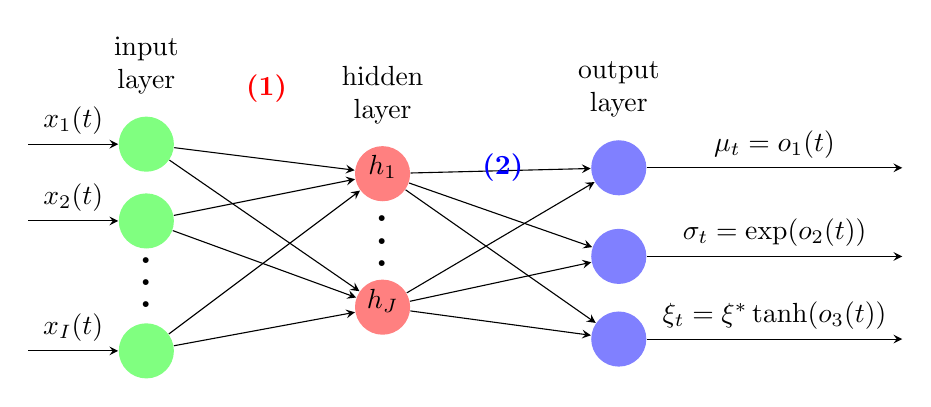
\begin{tikzpicture}[x=1.5cm, y=1.5cm, >=stealth]
				\tikzstyle{annot} = [text width=4em, text centered]
				
				\foreach \m [count=\y] in {1}
				\node [circle,fill=green!50,minimum size=.7cm ] (input-\m) at (0,1) {};
				
				\foreach \m [count=\y] in {2}
				\node [circle,fill=green!50,minimum size=.7cm ] (input-\m) at (0,0.35) {};
				
				\foreach \m [count=\y] in {3}
				\node [circle,fill=green!50,minimum size=.7cm ] (input-\m) at (0,-0.75) {};
				
				\node [neuron missing]  at (0,-0.25) {};
				
				\foreach \m [count=\y] in {1}
				\node [circle,fill=red!50,minimum size=.7cm ] (hidden-\m) at (2,0.75) {};
				
				\foreach \m [count=\y] in {2}
				\node [circle,fill=red!50,minimum size=.7cm ] (hidden-\m) at (2,-0.38) {};
				
				\node [neuron missing]  at (2,0.1) {};
				
				\foreach \m [count=\y] in {1}
				\node [circle,fill=blue!50,minimum size=.7cm ] (output-\m) at (4,1.8-\y) {};
				
				\foreach \m [count=\y] in {2}
				\node [circle,fill=blue!50,minimum size=.7cm ] (output-\m) at (4,1.05-\y) {};
				
				\foreach \m [count=\y] in {3}
				\node [circle,fill=blue!50,minimum size=.7cm ] (output-\m) at (4,0.35-\y) {};
				
				\draw [<-] (input-1) -- ++(-1,0)
				node [above, midway] {$\boldsymbol{x_1(t)}$};
				\draw [<-] (input-2) -- ++(-1,0)
				node [above, midway] {$x_2(t)$};
				\draw [<-] (input-3) -- ++(-1,0)
				node [above, midway] {$x_I(t)$};
				
				\node [below] at (hidden-1.north) {$h_1$};
				\node [below] at (hidden-2.north) {$h_J$};
				
				\draw [->] (output-1) -- ++(2.4,0)
				node [above, midway] {$\boldsymbol{\mu_t=o_1(t)}$};
				\draw [->] (output-2) -- ++(2.4,0)
				node [above, midway] {$\sigma_t=\exp(o_2(t))$};
				\draw [->] (output-3) -- ++(2.4,0)
				node [above, midway] {$\xi_t=\xi^*\tanh(o_3(t))$};
				
				\foreach \i in {1,...,3}
				\foreach \j in {1,...,2}
				\draw [->] (input-\i) -- (hidden-\j);
				
				\foreach \i in {1,...,2}
				\foreach \j in {1,...,3}
				\draw [->] (hidden-\i) -- (output-\j);
				
				\node[annot,above of=hidden-1, node distance=1cm] (hl) {hidden layer};
				\node[annot,above of=input-1] (il) {input layer};
				\node[annot,above of=output-1] {output layer};
				\node[annot, above =2.2cm, right=0.7cm, node distance=1cm]{\textcolor{red}{\textbf{(1)}}};
				\node[annot, above =1.2cm, right=3.7cm]{\textcolor{blue}{\textbf{(2)}}};
				\end{tikzpicture}
			}
		}
		\vspace{-2.5mm}
		\caption{\emph{ Neural Network applied to GEV. Figure made with \texttt{tikzpicture} and based on  \textcolor{JungleGreen}{\cite{cannon_flexible_2010}}} }. Here $x_i(t)=t,  \ \forall i \in \{1,\ldots,I\}$ 
	\end{center}
\end{figure}

\paragraph*{Parametric or nonparametric ?}
It is always a difficult task to state whether Neural Networks (NN) are parametric models or not. NN  are somewhere in the gray area between a \emph{parametric} and a \emph{nonparametric} model, in the sense that it assumes the GEV distribution from the output layer which are defined by the three parameters of interest, while it also allows for a fabulous flexibility coming from the hidden layers and which lead to think that these ae rather nonparametric. 

The transformations applied through the ntwork are in general parametric (and nonlinear).

However, this terminological question is actually not relevant here and it is more important to focus on the architecture of the NN employed here.

have the power to manage several outputs in a 

"Model parameters are estimated via the GML approach using the
quasi-Newton BFGS optimization algorithm, and the appropriate GEV-CDN model architecture for
each location is selected by fitting increasingly complicated models and choosing the one that
minimizes appropriate cost-complexity model selection criteria. For each location examined, different
formulations are tested with combinational cases of stationary and nonstationary parameters of the
GEV distribution, linear and nonlinear architecture of the CDN and combinations of the input covariates "


\cite{carreau_hybrid_2009} enlightens the following : Provided enough data, hidden units and an appropriate optimization, the NN can capture any smooth dependencies (relationships) of the parameters on the input, i.e., given the input, it can theoretically capture any conditional continuous density, be it asymmetric, \textbf{multimodal}, or heavy-tailed.

(see \citet{cannon_flexible_2010} just before conclusion) 
One could for example expect to have particular relationships between the covariate (time or) and the parameters of interest. Only considering a linear or quadratic trends in the location parameter $\mu$ (ore more ? see section. see for other parameters) could thus be seen as a weak modelling procedure, especially when we assumed no reliable prior knowledge on the subject (see bayesian section - hyperref it).
NN models have this facility of being capable of modelling any relationships without explicitly specify it \emph{a priori}. To model correctly, one should be able to explicitly discover particular patterns (e.g., which nonlinear or linear relationship between time and TN). This is avoided here because this is done automatically through the NN process.

Physical process such as temperature or even other meteorological data (rainfall as demonstrated by \citet{cannon_flexible_2010},...) have this tendance of demonstrating nonlinearities ( see ref?) and so are NN's interesting.

As we mentioned, the NN is meant to approximate any functions with good accuracy. It comprise thus all the models considered so far, such as linear tren din $\mu$, quadratic, etc...

\citet{cannon_flexible_2010} recommended to use between 1 and 3 (4) hidden layers due to the relatively small sample of annual extremes (here 117).


From this, we must pay attention to the high danger of \emph{overfitting} (see ) which occurs for this sort of models. The other pitfall is its lack of interpretation of the retrieved relationships.

"It bears noting that sensitivity analysis methods,
for example, the one used by Cannon and McKendry
(2002), are applicable to CDN models and could be used
to identify the form of nonlinear relationships between
covariates and GEV distribution parameters or quantiles."

... Intro to deep learning.. ?

\subsection{Bagging} 

Nowadays, bagging is used in 
many state-of-the-art algorithms such as Random Forests (see .. for comparisons of such techniques) and is one of the \emph{ensemble methods} which are praised in Machine Learning for their performance.  

In a "pure" climatological point of view, \emph{ensemble models} are of major utility, especially to make weather forecasting, see for example \citet{suh_development_2012} or, .... among others

For our purpose, we present another kind of ensemble modelling which is \emph{bagging}.

" Bagging (stands for Bootstrap Aggregation) is the way decrease the variance of your prediction by generating additional data for training from your original dataset using combinations with repetitions to produce multisets of the same cardinality/size as your original data. By increasing the size of your training set you can't improve the model predictive force, but just decrease the variance, narrowly tuning the prediction to expected outcome "


"model averaging, which involves taking a weighted average of
multiple models, has been recommended as a means of
improving estimation performance Burnham and Anderson, 2004. This approach has been applied successfully
in the context of CDN models by Carney et al. (2005)
and is worth exploring for GEV-CDN models."


\citet[pp.256-267]{Goodfellow-et-al-2016}  (deep learning html book)    The  individual  classifiers’  predictions  (having equal  weightage)  are  then  combined  by  taking  majority voting. This typically reduces the variance and then the (possible) overfitting



\subsubsection*{xxx}

"weight penalty regularization (MacKay, 1992) is
available as a means of limiting the effective number of model
parameters in a GEVcdn model. The amount of weight penalty is
controlled via a user-specified Gaussian prior on the magnitude of
the input-hidden layer weights. The optimum value for the
variance of the Gaussian prior must be set by the user with the
aid of some form of split-sample or cross-validation scheme." (cannon gevcdn vignette pdf)

\subsection{Bootstrap Methods in EVT}

" like
the estimated parameters themselves, the SE may not be
reliable for small samples. One way to tackle this problem and improve the accuracy of SE is through the bootstrap technique (Efron, 1979). The scheme for using this technique for EV dfs is described in detail by Katz et al. (2002), including for nonstationary cases,
in which the bootstrap samples are manufactured through
Monte  Carlo  resampling  of  residuals  (Equation (8))  to attend  to  the  underlying  assumption  that  original  sam-
ple  consist  of  iid  data.  Following  this procedure,  the bootstrap  procedure  was  designed  for  generating  1000
samples  from  each  original  sample,  considering  whole year  as  a  bloc"


In \citet{cannon_flexible_2010}, "he parametric bootstrap outperformed the residual bootstrap"
Moreover, " It is possible that alternative bootstrap approaches, for example, the bias-adjusted percentile estimators evaluated by Kysely
(2008), might yield better calibrated confidence intervals, although improvements were modest for stationary GEV models. "


For confidence intervals : see \citet[pp.681]{cannon_flexible_2010} 
following these steps

\begin{enumerate}
	\item Fit a nonstationary model to the data
	\item Transform the residuals from the fitted model so that they are identically distributed :
	\begin{equation}
	\varepsilon_t=\bigg[1+\xi_t\sigma^{-1}_t(y_t-\mu_t)\bigg]^{-\xi^{-1}}
	\end{equation}
	\item etc..
\end{enumerate}

Monte-Carlo based methods, same as Bayesian.

Study and comparisons on the performance (coverage,..) of the methods used for the CI (boot, bayesian, likelihood, asymptotics,...)

\subsubsection*{Moving Block Bootstrap}

[Bootstrap and other resampling in .... pp.13]


\subsection{Markov models}
book risk pp.136, \cite{shaby_markov-switching_2016} + code
